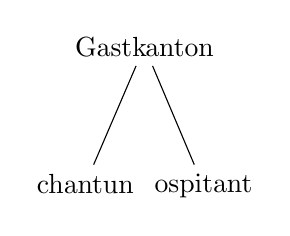
\begin{tikzpicture}
\node[align=left, anchor=north]{Gastkanton}
	child { node[anchor=north]{chantun}}
	child { node[anchor=north]{ospitant}}
;
\end{tikzpicture}

\begin{tikzpicture}
% First make a matrix containing as many columns as the longest sentence.
% Each cell contains a node whose label is identical to the word itself
\matrix[column sep=0em,row sep=.4in] {
% First sentence
\hnode{The} & \hnode{proposal} & \hnode{will} & \hnode{not} & \hnode{now} & \hnode{be} &  \hnode{implemented}  &\\
% Now create some dummy nodes to make intermediate nodes
& & & \node[inner sep={0pt},minimum width=0pt] (p1) {}; & & & \node[inner sep={0pt},minimum width=0pt] (p2) {};\\
% Second sentence
\hnode{Les} & \hnode{propositions} & \hnode{ne}  & \hnode{seront} & \hnode{pas} & \hnode{mises} & \hnode{en} & \hnode{application} & \hnode{maintenant}\\
};
% Now connect the nodes.  For paths that we want to break, name the path
\draw (The) -- (Les);
\draw (proposal) -- (propositions);
\draw[name path=willP] (will) -- (seront.north);
\draw (not) -- (p1);
\path[name path=neP] (p1) -- (ne);
\draw (p1) -- (pas);
\draw[name path=nowP] (now.south)  -- (maintenant.north);
\path[name path=impP] (implemented) -- (p2);
\draw (p2) -- (mises.north);
\draw (p2) -- (en);
\draw (p2) -- (application.north);
% Now break the paths at the intersection by drawing a white circle over it
\fill[white, name intersections={of=willP and neP}] (intersection-1) circle (4pt);
\fill[white, name intersections={of=nowP and impP}] (intersection-1) circle (4pt);
% Finally redraw the path you don't want broken
% Is there a more elegant way to do this?
\draw (p1) -- (ne);
\draw (implemented) -- (p2);
\end{tikzpicture}


\begin{tikzpicture}
% First make a matrix containing as many columns as the longest sentence.
% Each cell contains a node whose label is identical to the word itself

% First sentence
\hnode{nichtarbeitslose} \hnode{Stellensuchende} \\
% Now create some dummy nodes to make intermediate nodes
% & & & \node[inner sep={0pt},minimum width=0pt] (p1) {}; & & & \node[inner sep={0pt},minimum width=0pt] (p2) {};\\
% Second sentence
\hnode{persunas}  \hnode{che}  \hnode{tschertgan}  \hnode{ine}  \hnode{plazza}  \hnode{che} \hnode{n'}  \hnode{èn}  \hnode{betg}  \hnode{dischoccupadas}
;
% Now connect the nodes.  For paths that we want to break, name the path
\draw (nichtarbeitslose) -- (betg);
\draw (nichtarbeitslose) -- (dischoccupadas);
% Finally redraw the path you don't want broken
% Is there a more elegant way to do this?

\end{tikzpicture}

\begin{pspicture}(10,10)
  \rput[l](0,1){% English phrase
    \makebox[\widthof{Les propositions ne seront pas mises en application maintenant}][l]{\Tword{The} \Tword{proposal} \Tword{will} \Tword{not} \Tword{now} \Tword{be} \Tword{implemented}}%
  }%

    \rput[l](0,-1){% French phrase
    \Bword{Les} \Bword{propositions} \Bword{ne} \Bword{seront} \Bword{pas} \Bword{mises} \Bword{en} \Bword{application} \Bword{maintenant}%
  }%

  % Node connections between TOP (English) and BOTTOM (French) phrases
  \TtoB{The}{Les}%
  \TtoB{proposal}{propositions}%
  \TtoB{will}{seront}%
  \TtoB[linewidth=5pt]{not}{ne} \TtoB{not}{ne} \TtoB{not}{pas}%
  \TtoB{now}{maintenant}%
  \TtoB[linewidth=5pt,linecolor=white]{implemented}{mises}%
  \TtoB[linewidth=5pt,linecolor=white]{implemented}{en}%
  \TtoB[linewidth=5pt,linecolor=white]{implemented}{application}%
  \TtoB{implemented}{mises} \TtoB{implemented}{en} \TtoB{implemented}{application}% Redraw
\end{pspicture}


\rput(0,3){\rnode{A}{Foo}}
\rput(2,0){\rnode{B}{Bar}}
\ncdiag[angleA=-90,angleB=90,arm=5mm]{A}{B}
\hspace{2in}
\begin{tikzpicture}
\node at (0,0) (A) {Bar};
\node at (-2,3) (B) {Foo};
\draw[thick] (A) -- (B);
\end{tikzpicture}

\begin{figure}
\centering
        \tikzmarknode{HE}{He} \tikzmarknode{GAVE}{gave} \tikzmarknode{ME}{me} \tikzmarknode{THE}{the} \tikzmarknode{BOOK}{book}
        
        \vspace*{1cm}
        
        \tikzmarknode{HAN}{Han} \tikzmarknode{GAV}{gav} \tikzmarknode{BOKEN}{boken} \tikzmarknode{TILL}{till} \tikzmarknode{MIG}{mig}

    
    \begin{tikzpicture}[remember picture, overlay]
        \draw    (HE) -- (HAN)
                (GAVE) -- (GAV)
                (ME.south) -- (TILL)
                (ME.south) -- (MIG)
                (BOOK) -- (BOKEN.north);
        \draw[dashed]
                (THE) -- (BOKEN.north);
                
    \end{tikzpicture}
\caption{Example}
\end{figure}